\documentclass{article}

% Packages
% ---
\usepackage{amsmath,amssymb,amsthm} 	% Advanced math typesetting
% \usepackage[utf8]{inputenc} 	% Unicode support (Umlauts etc.)
\usepackage[USenglish]{babel} 	% Change hyphenation rules
\usepackage{hyperref} 				% Add a link to your document
\usepackage{graphicx}				% Add pictures to your document
\graphicspath{ {./images/} }	% image directory

% Typewriter settings for code
\usepackage{listings} 				% Source code formatting and highlighting
\lstset{basicstyle=\ttfamily}		%Typewriter font for code writing


\usepackage{enumitem}

% Margins
\usepackage{geometry}
\geometry{margin=1in}


\usepackage{float}
\restylefloat{figure}
\usepackage{mathabx}
\usepackage{fancyhdr}
\usepackage[dvipsnames]{xcolor}
\usepackage{scrextend}

% Siderules for digressions/examples
\usepackage{mdframed}
\newmdenv[
topline=false,
bottomline=false,
skipabove=\topsep,
skipbelow=\topsep
]{siderules}

% Colors
\definecolor{blu}{rgb}{0,0,1}
\def\blu#1{{\color{blu}#1}}
\definecolor{gre}{rgb}{0,.5,0}
\def\gre#1{{\color{gre}#1}}
\definecolor{red}{rgb}{1,0,0}
\def\red#1{{\color{red}#1}}
\def\norm#1{\|#1\|}


% Headers
\pagestyle{fancy}
\fancyhf{}
\lhead{\bf CPSC 322 \\ Week 10 }
\rhead{\bf Jeremi Do Dinh \\ 61985628}
\rfoot{Page \thepage}

% Graph drawing tools
\usepackage{tikz}						
\usetikzlibrary {positioning}

\usepackage{breqn}
\usepackage{multicol} 				% Multiple column functionality
\usepackage{blindtext}

% Figure shortcut
\newcommand{\centerfig}[2]{\begin{center}\includegraphics[width=#1\textwidth]{#2}\end{center}}

\begin{document}

\section*{Lecture 26 - Introduction to Belief Networks}
\url{https://www.cs.ubc.ca/~jordon/teaching/cpsc322/2019w2/lectures/lecture26.pdf}
\subsubsection*{Goals:}
\begin{itemize}
	\item Build a Belief Network for a simple domain
	\item Classify the types of inference
	\item Compute the representational saving in terms on number of probabilities required
\end{itemize}

\subsection*{Belief Networkse}
\begin{siderules}
\textbf{Burglary Example}\\
\\

Suppose we have the following scenario:
\begin{itemize}
	\item There might be a \textbf{\blu{B}}urglar in my house
	\item The \textbf{anti-burglar \blu{A}larm} in my house may go off
	\item I have an agreement with two of my neighbors, \textbf{\blu{J}ohn} and \textbf{\blu{M}ary}, that they \textbf{call} me if they hear the alarm go off when I am at work
	\item \textbf{Minor \blu{E}arthquakes} may occur and sometimes the set off the alarm.
	\item The \textbf{variables} are: \textbf{\blu{B, A, J, M, E}}
	\item \textbf{Joint} has entries/probabilities
\end{itemize}
In belief networks we typically order the variables to reflect on the casual knowledge:
\begin{itemize}
	\item A burglar (\textbf{\blu{B}}) can set the alarm (\textbf{\blu{A}}) off
	\item An earthquake (\textbf{\blu{E}}) can set the alarm (\textbf{\blu{A}}) off
	\item The alarm can cause Mary to call (\textbf{\blu{M}})
	\item The alarm can cause John to call (\textbf{\blu{J}})
\end{itemize}
\centerfig{0.3}{BN-1}
We can then apply the chain rule to the joint distribution:
\begin{align*}
	P(B, E, A, M, J) &= P(B)P(E|B)P(A|B,E)P(M|A, B ,E)P(J|M, A, E, B) \\
	\intertext{which lets us simlify based on the \blu{marginal} and {\color{orange} conditional} independence} 
	&= P(B)\blu{P(E)}P(A|B,E){\color{orange}P(M|A)P(J|A)}
\end{align*}
Consequently, we express the result as a network where:
\begin{itemize}
	\item Each variable is a node.
	\item For each variable, the conditioning variables are its parents.
	\item We associate to each node its corresponding conditional probabilities.
\end{itemize}
This yields a directed acyclic graph (\textit{DAG}). 
\end{siderules}
\subsubsection*{In general}
To define a belief network on a set of variables $ \{X_1, \dots, X_n\} $, first we need to select a definite ordering of the variables. Then we apply the chain rule, as discussed previously, where:
\begin{align*}
P(X_1 = v_1 \land \dots \land X_n = v_n)&= \prod_{i=1}^n P(X_i = v_i | X_1 = v_1 \land \dots \land X_{i-1} = v_{i-1})\\
\intertext{or in other terms:}
P(X_1, \dots, X_n)&= \prod_{i=1}^n P(X_i | X_1, \dots, X_{i-1})
\end{align*}
We subsequently define the parents of a random variable, $ \text{parents}(X_i) $ to be the minimal number of predecessors of $ X_i $ in the total ordering, such that the other predecessors of $ X_i $ are conditionally independent of $ X_i $ given parents$ (X_i) $. In other words, this means that $ X_i $ probabilistically depends on its parents, but is independent of its other predecessors. This means that: parents$ (X_i) \subset\{X_1, \dots, X_{i-1}\} $ such that:
\begin{align*}
P(X_i | X_1, \dots, X_{i-1}) &= P(X_i | \text{parents}(X_i))
\end{align*}
There can be several numbers of \textit{minimal} sets which may be defined as predecessors satisfying this condition, and any one of those may be chosen to be a parent. There can be more than one minimal set only when some of the predecessors are deterministic functions of others.\\
\\
The chain rule a result is re-written as follows:
\begin{align*}
P(X_1, \dots, X_n)&= \prod_{i=1}^n P(X_i | \text{parents}(X_i))
\end{align*}
A belief network as a result defines a \textbf{factorization} of the joint probability distribution into a product of conditional probabilities. A belief network may be referred to as a \textbf{\textit{Bayesian}} network, and it is a DAG where (as described above) the nodes are random variables, there is an arc from each of the elements of parents$ (X_i) $ to $ X_i $.\\
\\
We have that each node is independent from its \textit{non-descendants} given its parents. A node is independent from the rest of the network given its \textit{Markov blanket}, which in this case would be its set of parents.\\
\\
A belief network has an associated set of conditional probability distributions that specify the probability of each variable given its parents (which includes the prior probabilities of those variables with no parents). \\
\\
We also have that different ordering will result in different decompositions, as well as even fewer decompositions, and graphs which involve less arcs. 

\subsubsection*{Compactness}
A \textbf{Conditional probability table (CPT)} for \textbf{\blu{boolean}} $ X_i $ with $ k $ \textbf{\blu{boolean}} parents had \blu{$ 2^k $} rows for the combinations of the parent values. Each row requires \textbf{one number} $ p_i $ to represent $ X_i =  $ true (the conjugate of which would be $ 1 - p_i $ to represent $ X_i =$ false). \\
\\
If each variable has no more than $ k $ parents, then the complete network requires $ O(n2^k) $ numbers to represent. If $ k << n $, then this is a vast improvement from the previous space complexity of $ O(2^n) $ 
\newpage
\section*{Lecture 27 - Belief Networks continued}
\url{https://www.cs.ubc.ca/~jordon/teaching/cpsc322/2019w2/lectures/lecture27.pdf}
\subsubsection*{Open Issues:}
Following the previous section, we are still left with a number of issues that occur:
\begin{itemize}
	\item \textbf{Independencies}: Does a BNet encode more independencies than the ones specified by construction? \quad \textit{Yes}
	\item \textbf{Compactness}: We reduce the number of probabilities from $ O(2^n) $ to $ O(n2^k) $. \\
	However in some domains we may need to do better than that. 
	\item Still too many and often there are no data/experts for accurate assessment
\end{itemize}
The \textbf{solution} is to make stronger (approximate) \textbf{independence assumptions}. 

\subsection*{Conditional Independencies/Dependencies with common ancestors}
In certain cases, we have that two variables' dependency will depend on the value observed of other variables. \\
\begin{siderules}
\textbf{Example 1}\\
\\
Consider the following example of a snapshot of a belief network:
\centerfig{0.4}{BN-2}
We have that:
\begin{itemize}
	\item \textsl{Alarm} and \textsl{Smoke} are dependent, \textbf{however}
	\item  \textsl{Alarm} and \textsl{Smoke} are independent given \textsl{Fire}
	\item Intuitively, \textsl{Alarm} can explain \textsl{Alarm} and \textsl{Smoke}; thus learning from one can affect the other by changing the belief in \textsl{Fire}.
\end{itemize}
\textbf{Example 2}\\
\\
Another scenario can be pictured with the following example:
\centerfig{0.25}{BN-3}
In this case we have that:
\begin{itemize}
	\item \textsl{Alarm} and \textsl{Report} are dependent
	\item \textsl{Alarm} and \textsl{Report} are independent given \textsl{Leaving}
	\item Intuitively, the only way that the \textsl{Alarm} affects \textsl{Report} is by affecting \textsl{Leaving}.
\end{itemize}
\textbf{Example 3}\\
\\
Lets take yet another example:
\centerfig{0.35}{BN-5}
Here we have that;
\begin{itemize}
	\item \textsl{Tampering} and \textsl{Fire} are independent
	\item \textsl{Tampering} and \textsl{Fire} are dependent given \textsl{Alarm}
	\item Intuitively, \textsl{Tampering} can explain away \textsl{Fire}
\end{itemize}
\end{siderules}
\subsection*{Understanding independence}
In general there's three ways in which there can be a block in terms of probability propagation. Those are illustrated in the figure below, with 3 different paths, involving variables in subsets X, Y and Z:
\subsubsection*{Conditional Independencies}
\centerfig{0.9}{BN-6}
\begin{itemize}
	\item In paths 1 and 2, those paths become blocked as soon as we observe evidence \textbf{E}.
	\item In path 3, $ X $ and $ Y $ become dependent as soon as we get evidence for $ Z $, or any of its descendants.
	\item Otherwise, X and Y remain independent if evidence is observed as shown above.
\end{itemize}
\subsubsection*{Conditional Dependencies}
The following diagram represents cases where new evidence will cause variables to become dependent (i.e.: the opposite of the above example):
\centerfig{0.9}{BN-7}
These are cases where X and Y are conditionally dependent on each other\\
\\
\subsubsection*{Conditional Dependencies}
In general we have the following rules:
\begin{itemize}
	\item If we observe variable(s) $ \bar{Y} $, the variables whose posterior probability is different from the prior are:
	\begin{itemize}[label=$\rightarrow$]
		\item The ancestors of $ \bar{Y} $
		\item The descendants of the ancestors of $\bar{Y}$
	\end{itemize}
\item Intuitively, if we have a causal belief network:
\begin{itemize}[label=$\rightarrow$]
	\item We do \red{abduction} to possible causes
	\item \red{prediction} from the causes
\end{itemize}
\end{itemize}
%\centerfig{0.8}{BN-4}
%We can ask the following questions:
%\begin{enumerate}
%	\item On which given probabilities does $ P(N) $ depend?
%	\item If you were to observe a value for $ B $, which variables’probabilities will change?
%	\item If you were to observe a value for $ N $, which variables’ probabilities will change?
%	\item Suppose you had observed a value for $ M $; if you were to then observe a value for $ N $, which variables’ probabilities will change?
%	\item Suppose you had observed $ B $ and $ Q $; which variables’ probabilities will change when you observe $ N $?
%\end{enumerate}


\subsection*{Compact Conditional Distributions}
Once we have constructed the topology (structure) of a belief network, we still need to specify the conditional probabilities. This can be done using the \textbf{data} of using information from \textbf{experts}. To facilitate acquisition, we aim for compact representations for which data/experts can provide accurate assessments.\\
\\
We observed that the Joint Probability table (JPT) has a size of $ O(2^n) $, where $ n $ is the number of binary variables. We have that the Conditional Probability Table (CPT) has a size of $ O(n2^k) $, where $ k $ is the maximum number of parents. \\
\\
However this is still a problem, given the fact that the CPT size grows exponentially with the number of parents. 

\subsubsection*{Effect with multiple non-interacting causes}
Suppose we want to investigate the effect of multiple non-interacting causes. This is illustrated by the diagram below:
\centerfig{0.5}{BN-8}
The green rown in the following table are the probabilities that experts would we able to easily provide:
\centerfig{0.6}{BN-9}
However it is more difficult to assess more complex conditioning. \\
\\
\textbf{The solution} is \textbf{\textit{Noisy OR- Distributions}}
This type of distribution:
\begin{itemize}
	\item Models multiple non-interacting causes
	\item Uses logical OR with a probabilistic twist. 
	\item A logic or conditional probability table is illustrated below:
	\centerfig{0.6}{BN-10}
\end{itemize}
The noisy OR-model allows uncertainty in the ability of each cause to generate an effect (for example how one may have a cold without a fever). For this we have \textbf{two assumptions}:
\begin{itemize}
	\item All possible causes are listed
	\item For each of the causes, whatever \textbf{\blu{inhibits}} it to generate an effect is \textit{independent} from the \textbf{\blu{inhibitors}} of the other causes.
\end{itemize}
\begin{center}

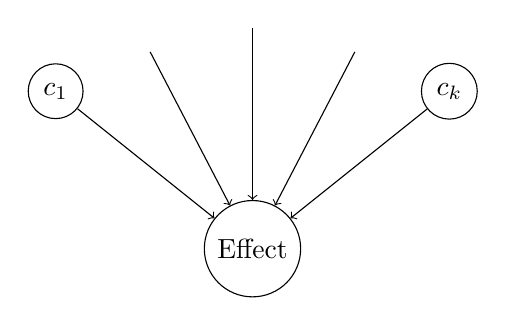
\begin{tikzpicture}

\node[shape=circle,draw=black] (1) at (0,3) {$ c_1 $};
%\node[shape=circle,draw=black] (i) at (2.5,4) {$ c_i $};
\node[shape=circle,draw=black] (e) at (2.5,1) {Effect};
\node[shape=circle,draw=black] (k) at (5,3) {$ c_k $} ;


\path [->] (1) edge node[left] {} (e);
\path [->](2.5,3.8) edge node[left] {} (e);
\path [->](k) edge node[left] {} (e);
\path [->](1.2, 3.5) edge node[left] {} (e);
\path [->](3.8, 3.5) edge node[left] {} (e);

\end{tikzpicture}
\end{center}
Suppose in the diagram above we have the the causes $ c_1, \dots, c_k $, which each have a probability of failure to trigger the effect of $ q_i $, with $ i \in \{1, \dots, k\} $. Then we have that:
\begin{itemize}
	\item $ P(\text{Effect }= F | C_i = T, \text{and no other causes}) = q_i$
	\item $ P(\text{Effect }= \red{F} | {\color{Fuchsia}C_1 = T, \dots, C_j = T}, C_{j+1} = F, \dots, C_k = F) = \prod_{i = 1}^{j}q_i$
	\item $ P(\text{Effect }= \red{T} | {\color{Fuchsia}C_1 = T, \dots, C_j = T}, C_{j+1} = F, \dots, C_k = F) = 1 -  \prod_{i = 1}^{j}q_i$
\end{itemize}
\begin{siderules}
	We go back to the disease example, where we wish to fit the table of probabilities, given only a subset of the probabilities, and using the assumptions. We are given that:
	\begin{itemize}
		\item $ P(\text{Fever} = F | \text{Cold} = T, \text{Flu} = F, \text{Malaria} = F) = 0.6 $
		\item $ P(\text{Fever} = F | \text{Cold} = F, \text{Flu} = T, \text{Malaria} = F) = 0.2 $
		\item $ P(\text{Fever} = F | \text{Cold} = F, \text{Flu} = F, \text{Malaria} = T) = 0.1 $
	\end{itemize}
Then according to our above assumption that:
\begin{align*}
P(\text{Effect }= \red{F} | {\color{Fuchsia}C_1 = T, \dots, C_j = T}, C_{j+1} = F, \dots, C_k = F) = 1 -  \prod_{i = 1}^{j}q_i
\end{align*}
We can fill in the table as follows:
\begin{center}
	\begin{tabular}{|c|c|c|c|c|}
		\hline
		Malaria & Flu & Cold & $ P(\text{Fever}=T | ..) $ & $ P(\text{Fever}=F|..) $ \\
		\hline
		T & T & T& & $ 0.6 \cdot 0.2 \cdot 0.1 = 0.012 $  \\
		\hline
		T & T & F & & $ 0.2 \cdot 0.1 = 0.02 $ \\
		\hline
		T & F & T& & $ 0.6 \cdot 0.1 = 0.06 $ \\
		\hline
		T & F & F & \blu{$ 0.9 $} & \blu{$ 0.1 $} \\
		\hline
		F & T & T & & $ 0.2 \cdot 0.6 = 0.12 $ \\
		\hline
		F & T & F & \blu{$ 0.8 $} & \blu{$ 0.2$} \\
		\hline
		F & F & T & \blu{$ 0.4 $} & \blu{$ 0.6 $} \\
		\hline
		F & F & F & & 1.0\\
		\hline
	\end{tabular}
\end{center}
In internal medicine using these kinds of assumptions can have us go from 133,931,430 probabilities to just 8,254
\end{siderules}

\subsection*{Naïve Bayesian Classifier}
The Naïve Bayesian classifier is a very simple and successful Belief Network that allows us to classify \blu{entities} into a \blu{set of classes} $ C $, given a \blu{set of attributes}. \\
\\
Email Spam filtering is a classic example of that:
\begin{itemize}
	\item Determine whether an \textbf{email} is spam  ( we only have two classes $ spam =$ T and $ spam= $ F)
	\item We have that the useful attributes of the email are the \textbf{words} it contains
\end{itemize}
For this we make the following assumptions:
\begin{itemize}
	\item The value of each attribute depends on the classification
	\item (Naïve) The attributes are independent of each other given the classification
\end{itemize}
If we have a large collection of emails, of which we know the labels (spam vs. not spam) then for each word in the English dictionary, we can compute the probability of the email containing that word, given that it's spam. \\
\\
Bayes can then be used to predict on new emails, of which we do not know the label, if a email is spam or not, given the words it contains. The we classify that an email is spam if:
\begin{align*}
P(\text{spam} = T | \text{words it contains}) \ge P(\text{spam} = F | \text{words it contains})
\end{align*}
\centerfig{0.75}{BN-11}
With this type of parameters, we have that the joint probability distribution would have a space complexity around $ O(2^{10^5}) $ as opposed to $ O(2*10^5) $ for the model described here (assuming that there are approximately $ 10^5 $ words in the English dictionary).

\subsection*{Summary of Compactness}
In summary, we have discussed several methods where with $ n $ Boolean variables and at most $ k $ parents we can change the space complexity of our probabilities. Those are shown in the following figure:
\centerfig{0.8}{BNet-1}
\end{document}